\documentclass[12pt]{article}

\usepackage{amsmath, amsfonts, amssymb, amsthm}
\usepackage{graphicx, float}
\graphicspath{{images/}}

% Customization --------------

% GEOMETRY
% Sets paper size, margins, and a paramter.
\usepackage[
    letterpaper, 
    top = 0.8 in,
    bottom = 0.8 in,
    left = 1.0 in,
    right = 1.0 in,
    heightrounded
]{geometry}

% Line Height
\renewcommand{\baselinestretch}{1.15} % Line Spacing

%Parskip and Parindent
\setlength{\parindent}{0pt}
% \setlength{\parskip}{0.8em}

% End Customization ----------------

\title{\LaTeX \ Test}
\author{Caden Williamson}
\date{\today}


\begin{document}

\maketitle

\section{Introduction}
A short summary to make the rest sound interesting and important.

\subsection{Math}
In 1902, Einstein created this equation:
\begin{equation} \label{Theory of Relativity}
    E=mc^2
\end{equation}


Newton came up with this one: 
\begin{equation} \label{Force Equation}
    \sum F=ma
\end{equation}

\begin{equation} \label{Circle Area}
    \begin{split}
        A & = \frac{\pi r^2}{2} \\
        A & = \frac{2}{2} \pi r^2
    \end{split}
\end{equation}


\begin{figure}[H]
    \centering
    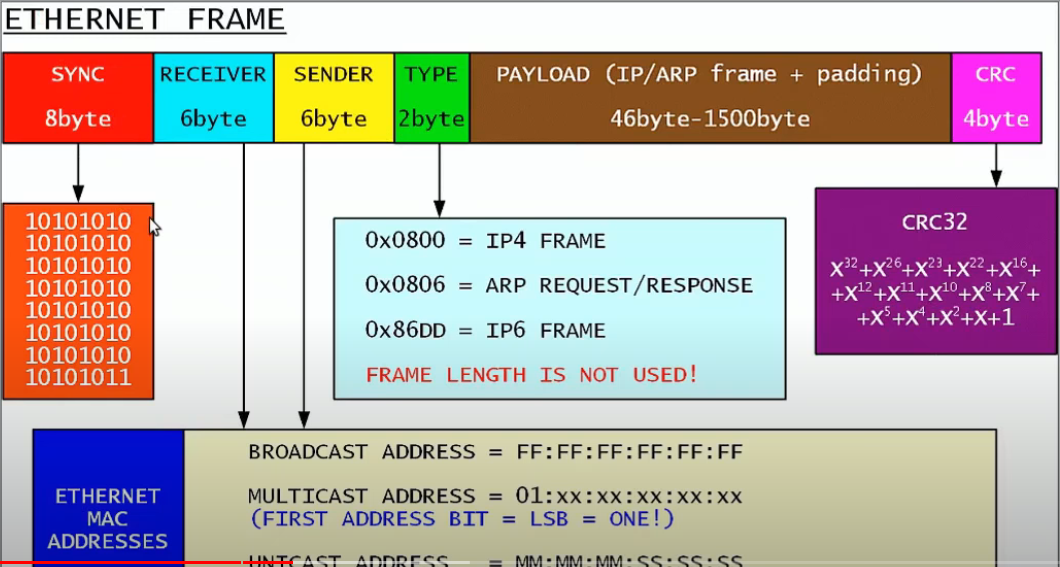
\includegraphics[width=5.5in]{EthernetFrame.png}
    \caption{My Caption}
\end{figure}

\end{document}